\begin{figure}
  \caption{Dependence of average net payoff ($\langle \pi \rangle$) at the
    end of last time step of the simulation on environmental
    variability $u$ for several values of low payoff $\pilow$, number of
    behaviors $B$, and lifespan $L$. Dashed lines mark expected 
    payoff from individual learning $\langle \pi_I \rangle$ calculated
    for each parameter setting (not sensitive to $u$). 
    Note that when the maximum $L$ is 
    8, the y-axis runs from 0 to 8, and when the maximum $L$ is 20, the y-axis
    runs from 0 to 20. Average over 1000 trials.} 
  \label{fig:meanNetPayoffs}
  \vspace{3em}
  % $\langle s \rangle$ decreases monotonically for $\pisub{low} = 0.1, 0.5$,
% but noise dominates the results for $\pisub{low}=0.8$. When $\pisub{low} = 0.5$, 
% the sigmoid is not as sharp as for $\pisub{low}=0.1$, meaning that social learning
% is reduced for smaller $u$ and increased for larger $u$.}
  \centering
  \addtocounter{figure}{-1}  % Hack to get figure numbering correct with subfigure.
  \begin{subfigure}[t]{0.08\textwidth}
    \vspace{-2em}
    \hspace{-4em}
    % \centering
    \begin{tikzpicture}
      \draw[->,thick] (-.1,0)--(1,0) node[above]
        {$B$};
        % {Number of behaviors $B$};
      \draw[->,thick] (0,.1)--(0,-1) node[below]
        {$\pilow$};
        % {Low payoff frequency $\pilow$};
    \end{tikzpicture}

  \end{subfigure}%
  \begin{subfigure}[t]{0.3\textwidth}
    \centering
    {\large $B = 2$} 
    \begin{rotate}{90}
      {\parbox{4cm}{
          \centering
          \vspace{-3.5em}{\large $ \pilow = 0.1$} \\
          {\begin{rotate}{-90}{\large $\langle \pi \rangle$}\end{rotate}}
      }}
    \end{rotate}%
    % \begin{rotate}{90}
    %   Social learning $\langle \pi \rangle$
    % \end{rotate}%
    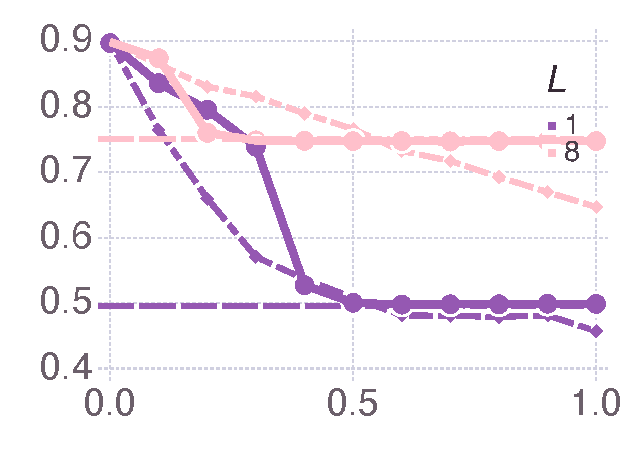
\includegraphics[width=1.1\textwidth]{
      {Figures/mean_prev_net_payoff_over_u_lowpayoff=0.1_nbehaviors=2.pdf}
    }
    \centering
    \begin{rotate}{90}
      {\parbox{4cm}{
          \centering
          \vspace{-3.5em} {\large$ \pilow = 0.45$} \\
          {\begin{rotate}{-90}{\large $\langle \pi \rangle$}\hspace{1em}\end{rotate}}
      }}
    \end{rotate}%
    % \hspace{1.5em}%
    % \begin{rotate}{90}
    %   Social learning $\langle \pi \rangle$
    % \end{rotate}%
    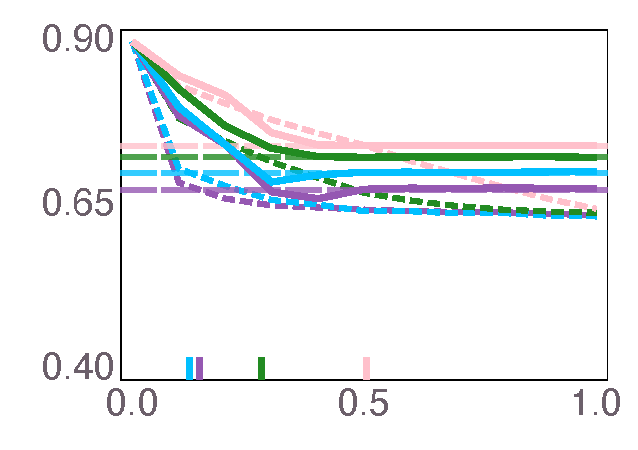
\includegraphics[width=1.1\textwidth]{
      {Figures/mean_prev_net_payoff_over_u_lowpayoff=0.45_nbehaviors=2.pdf}
    }
    \begin{rotate}{90}
      {\parbox{4cm}{
          \centering
          \vspace{-3.5em} {\large $ \pilow = 0.8$} \\
          {\begin{rotate}{-90}{\large $\langle \pi \rangle$}\end{rotate}}
      }}
    \end{rotate}%
    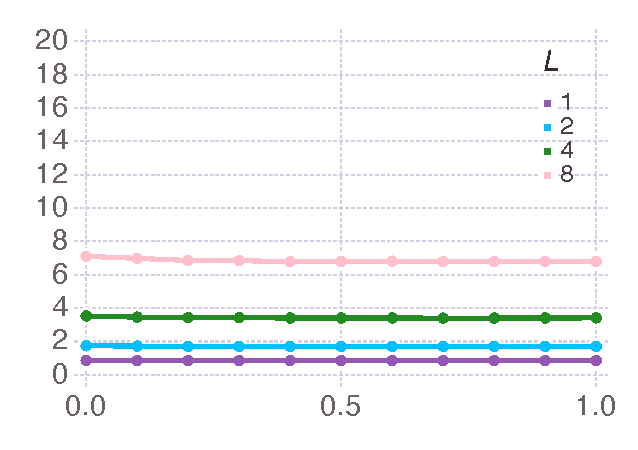
\includegraphics[width=1.1\textwidth]{
      {Figures/mean_prev_net_payoff_over_u_lowpayoff=0.8_nbehaviors=2.pdf}
    }\\[-.5em]
    {\large $\quad u$}
  \end{subfigure}%
  \begin{subfigure}[t]{0.3\textwidth}
    {\large $B = 4$}
    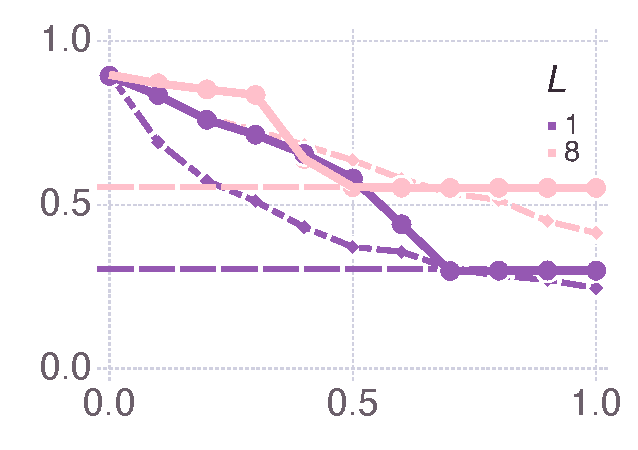
\includegraphics[width=1.1\textwidth]{
      {Figures/mean_prev_net_payoff_over_u_lowpayoff=0.1_nbehaviors=4.pdf}
    } \\
    \centering
    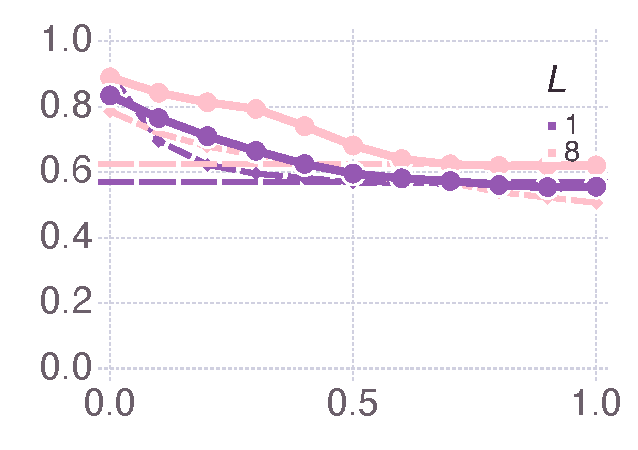
\includegraphics[width=1.1\textwidth]{
      {Figures/mean_prev_net_payoff_over_u_lowpayoff=0.45_nbehaviors=4.pdf}
    } \\
    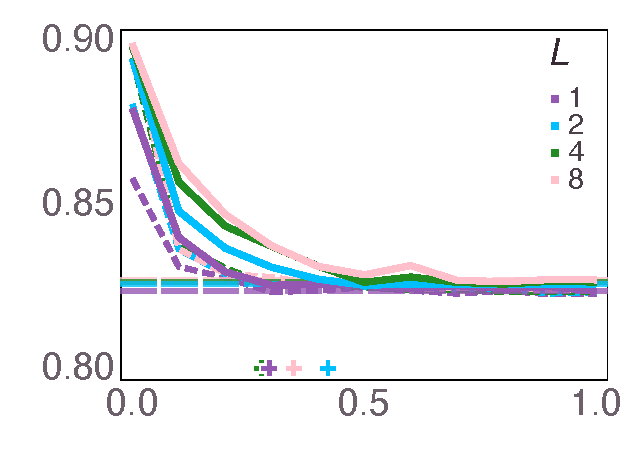
\includegraphics[width=1.1\textwidth]{
      {Figures/mean_prev_net_payoff_over_u_lowpayoff=0.8_nbehaviors=4.pdf}
    }\\[-.5em]
    {\large{$\quad u$}}
  \end{subfigure}
  \begin{subfigure}[t]{0.3\textwidth}
    \centering
    {\large $B = 10$}
    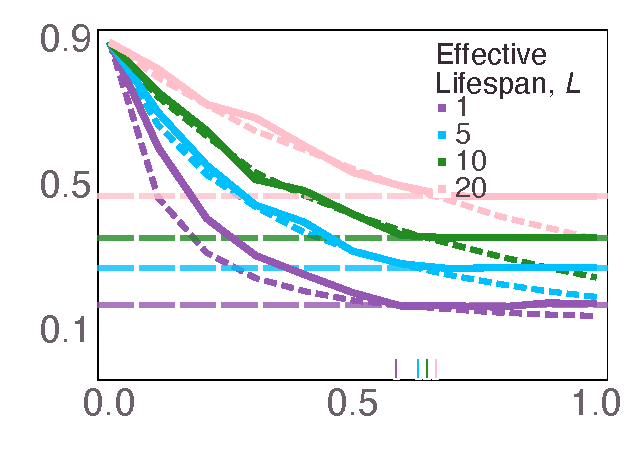
\includegraphics[width=1.1\textwidth]{
      {Figures/mean_prev_net_payoff_over_u_lowpayoff=0.1_nbehaviors=10.pdf}
    } \\
    \centering
    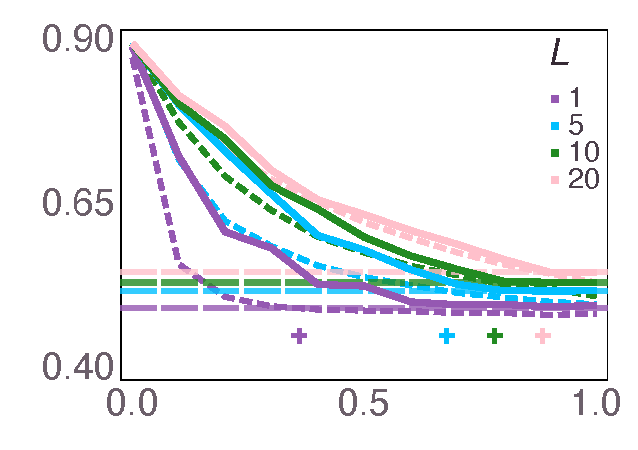
\includegraphics[width=1.1\textwidth]{
      {Figures/mean_prev_net_payoff_over_u_lowpayoff=0.45_nbehaviors=10.pdf}
    } \\
    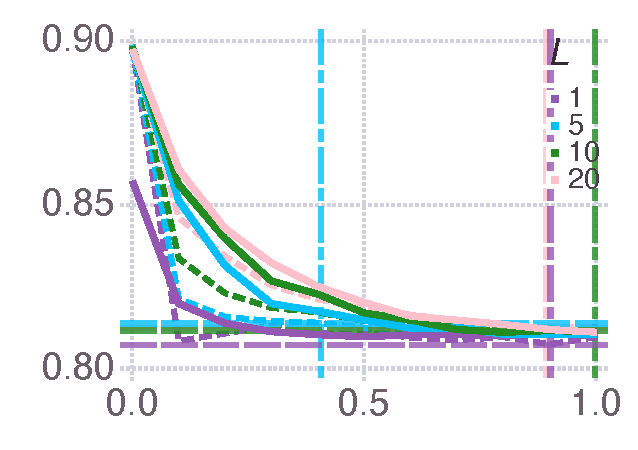
\includegraphics[width=1.1\textwidth]{
      {Figures/mean_prev_net_payoff_over_u_lowpayoff=0.8_nbehaviors=10.pdf}
    } \\[-.5em]
    {\large $\quad u$}
  \end{subfigure}
  
  
\end{figure}
